\documentclass[conference]{IEEEtran}

\usepackage{newtxtext}
\usepackage{amsmath}
\usepackage{newtxmath}
\usepackage{booktabs}
\usepackage{graphicx}
\usepackage{tabularx}
\usepackage{array}
\usepackage{cite}
\usepackage[hidelinks]{hyperref}
\usepackage{microtype}

\graphicspath{{../../results/figures/corrected_baseline/}}
\newcolumntype{Y}{>{\raggedright\arraybackslash}X}
\newcommand{\tps}{\mathrm{TPS}}
\newcommand{\ttft}{\mathrm{TTFT}}
\newcommand{\tpot}{\mathrm{TPOT}}

\title{Workload-Shaped Serving Optimization for\\
SmolLM2-360M on CPU and RTX 6000 Ada}

\author{
\IEEEauthorblockN{Hanxiao \qquad Haiyang Peng}
\IEEEauthorblockA{DSAA4012 Final Project}
}

\begin{document}
\maketitle

\begin{abstract}
We characterize how batch size and context length reshape the
time-to-first-token (TTFT), time-per-output-token (TPOT), throughput, and
memory frontier of SmolLM2-360M-Instruct. A deterministic manual decode loop
separates prefill from steady decode on one AMD EPYC 9654 socket and one
NVIDIA RTX 6000 Ada GPU. We then evaluate scaled-dot-product attention
(SDPA), key-value (KV) caching, and dynamic W8A8 quantization. The result is
conditional rather than universal. SDPA becomes increasingly valuable at
long context. Cache bookkeeping can slightly hurt the smallest GPU loads,
but avoiding the cache becomes 4.22$\times$ slower at context 2048, batch 8.
CPU W8A8 improves throughput by 1.27--2.49$\times$, yet increases peak
resident memory and severely degrades perplexity and ARC-Easy accuracy.
Correcting the benchmark to retain only final-position logits also removes
artificial out-of-memory boundaries, demonstrating that measurement
semantics are part of the systems result.
\end{abstract}

\begin{IEEEkeywords}
language-model serving, TTFT, TPOT, batching, attention, KV cache,
quantization
\end{IEEEkeywords}

\section{Problem and System Overview}

Serving optimization is often reduced to one tokens-per-second number. That
summary hides a multi-objective problem: a serving path must balance prefill
latency, decode latency, aggregate throughput, memory capacity, and output
quality. Our primary question is therefore a frontier question:
\emph{how do batch size and context length reshape the TTFT--TPOT--throughput
frontier, and when do attention, caching, and quantization move it?}

The model is \texttt{HuggingFaceTB/SmolLM2-360M-Instruct}, a compact
decoder-only Llama-family model from the SmolLM2 family~\cite{smollm2}. The
checked artifact contains 361,821,120 parameters, 32 decoder layers, hidden
size 960, intermediate size 2560, 15 query heads, 5 KV heads, grouped-query
attention, and an 8192-token maximum context. The small model is deliberate:
at small batch it is unlikely to saturate a high-end GPU, making framework
overhead, dispatch, bandwidth, attention, and matrix-throughput transitions
visible within a tractable experiment budget.

The study has two independent hardware lines. The CPU line uses logical CPUs
0--95 from one AMD EPYC 9654 NUMA/socket side, with 96 intra-op threads, one
inter-op thread, and FP32 weights. The GPU line uses only GPU0 of an
eight-GPU host: one RTX 6000 Ada with 48~GB memory and BF16 weights. Absolute
CPU and GPU results are not treated as a fairness comparison; we compare
scaling behavior and normalized intervention effects within each line.

\section{Design}

\subsection{Timing Boundaries and Metrics}

The benchmark separates autoregressive inference into prefill and decode.
Prefill consumes a prepared prompt and ends when the first generated token is
available. Decode then performs one forward step per sequence and generates
64 output tokens synchronously with greedy selection. Input construction,
tokenization, and terminal output are outside the measured region. CUDA is
synchronized at every token boundary.

For a generation producing $N$ tokens, model-only TTFT is the elapsed time
from the first model call to availability of the first generated token.
Steady decode latency is
\begin{equation}
\tpot = \frac{t_{\mathrm{last}}-t_{\mathrm{first}}}{N-1},
\end{equation}
and aggregate output-token throughput is
\begin{equation}
\tps = \frac{B N}{t_{\mathrm{last}}-t_{\mathrm{start}}},
\end{equation}
where $B$ is batch size. Prompt tokens are excluded from decode TPS. GPU peak
allocated and reserved memory and fresh-process CPU peak RSS are recorded.

\subsection{Workload Grid and Statistical Protocol}

Baseline grids span contexts $\{128,512,2048,4096\}$, CPU batches
$\{1,2,4,8,16\}$, and GPU batches
$\{1,2,4,8,16,32,64,128\}$. Each broad-grid point has ten measured
repetitions after warmup. Two GPU headline points, 128/1 and 4096/128, have
100 repetitions collected in ten alternating-order blocks. We report
median, p95, and p99, but use the 100-repetition files for stable tail claims.

The batching knee is frozen before analysis: it is the first tested batch
increase for which aggregate TPS improves by less than 10\% while p95 TTFT
or TPOT continues to rise. If no tested point meets the rule, we state that
no knee was observed rather than extrapolating one.

\subsection{Interventions and Quality}

We compare PyTorch eager attention with SDPA. PyTorch SDPA can dispatch to
fused backends~\cite{pytorch_sdpa}; CUDA profiling verifies that our selected
path executes \texttt{pytorch\_flash::flash\_fwd\_kernel}, consistent with
the IO-aware design principles of FlashAttention~\cite{flashattention}.
Eager profiles instead expose explicit batched matrix multiplies and
softmax.

KV cache enabled and disabled are compared at representative context/batch
points. Dynamic W8A8 quantization is evaluated on CPU with 224 Transformer
linear modules quantized and \texttt{lm\_head} retained in FP32. Quality is
measured with a frozen 12,846-token WikiText-2 slice~\cite{wikitext}, full
ARC-Easy~\cite{arc}, and full HellaSwag~\cite{hellaswag}.

\section{Implementation}

\subsection{Reproducible Harness}

The repository provides YAML-composed configurations, deterministic prompt
construction, a manual prefill/decode loop, token-level timing, memory
measurement, JSONL schema validation, resume-safe manifests, aggregation,
plotting, and quality-evaluation scripts. Each result records the merged
configuration, exact software versions, local model hashes, Git revision,
and invocation history. The final repository passes 22 model-free unit tests
and Ruff static checks.

\subsection{Correctness Boundary: Final-Position Logits}

An early implementation materialized full-sequence logits with shape
$[B,L,V]$ during prefill, even though greedy serving uses only the last
position. The corrected schema-v3 benchmark requests
\texttt{logits\_to\_keep=1}, producing $[B,1,V]$ on every forward. Legacy
records remain explicitly labeled \texttt{full\_logits\_prefill} and are
never combined with corrected aggregates.

This correction materially changes the measured memory boundary. Former OOM
points at 2048/128 and 4096/64 succeed in fresh processes and each uses about
16.33~GiB peak allocated memory. The 4096/128 point also succeeds at
31.95~GiB. Residual memory beyond weights and KV state scales with
$B\times L$, consistent with transient prefill QKV and MLP activations rather
than unused vocabulary logits. The correction is therefore not merely an
implementation detail; it changes which workloads appear feasible.

\subsection{Validation and Interpretation Discipline}

The corrected baseline contains 200 CPU and 320 GPU observations. Operator
experiments cover five representative points per hardware line with ten
repetitions per implementation. Cache experiments use repeated points except
for one explicitly labeled CPU boundary. Hardware, environment, test, lint,
telemetry, profiler, raw, processed, and plot artifacts are committed
together.

A faster quantized result is not attributed to INT8 without checking the
executed kernel. A slower quantized path is retained and analyzed. Memory
claims distinguish GPU allocator statistics from fresh-process CPU RSS.
Broad-grid p99 values based on ten repeats are descriptive only. Block
telemetry spans 29--70$^\circ$C without progressive failure or a memory leak.

\section{Evaluation}

\subsection{Baseline Surface}

Fig.~\ref{fig:baseline} shows the corrected median decode-TPS surfaces. CPU
median TPS peaks at 146.96, 119.91, 50.95, and 25.01 for contexts 128, 512,
2048, and 4096, respectively. The knee rule finds batch 16 at context 2048
and batch 8 at context 4096; no knee appears through batch 16 at contexts 128
or 512.

GPU median TPS reaches 2973.59, 2947.87, 2700.83, and 1437.52 at batch 128
for the same four contexts. Only context 4096 reaches the frozen knee at
batch 128. The other contexts still scale within the tested range. The
100-repetition 128/1 point has p50/p95/p99 TTFT of
41.54/44.08/44.67~ms. At 4096/128 these values are
6.745/6.899/6.923~s; p99 TPOT is 89.48~ms.

\begin{figure*}[t]
  \centering
  \begin{minipage}[t]{0.49\textwidth}
    \centering
    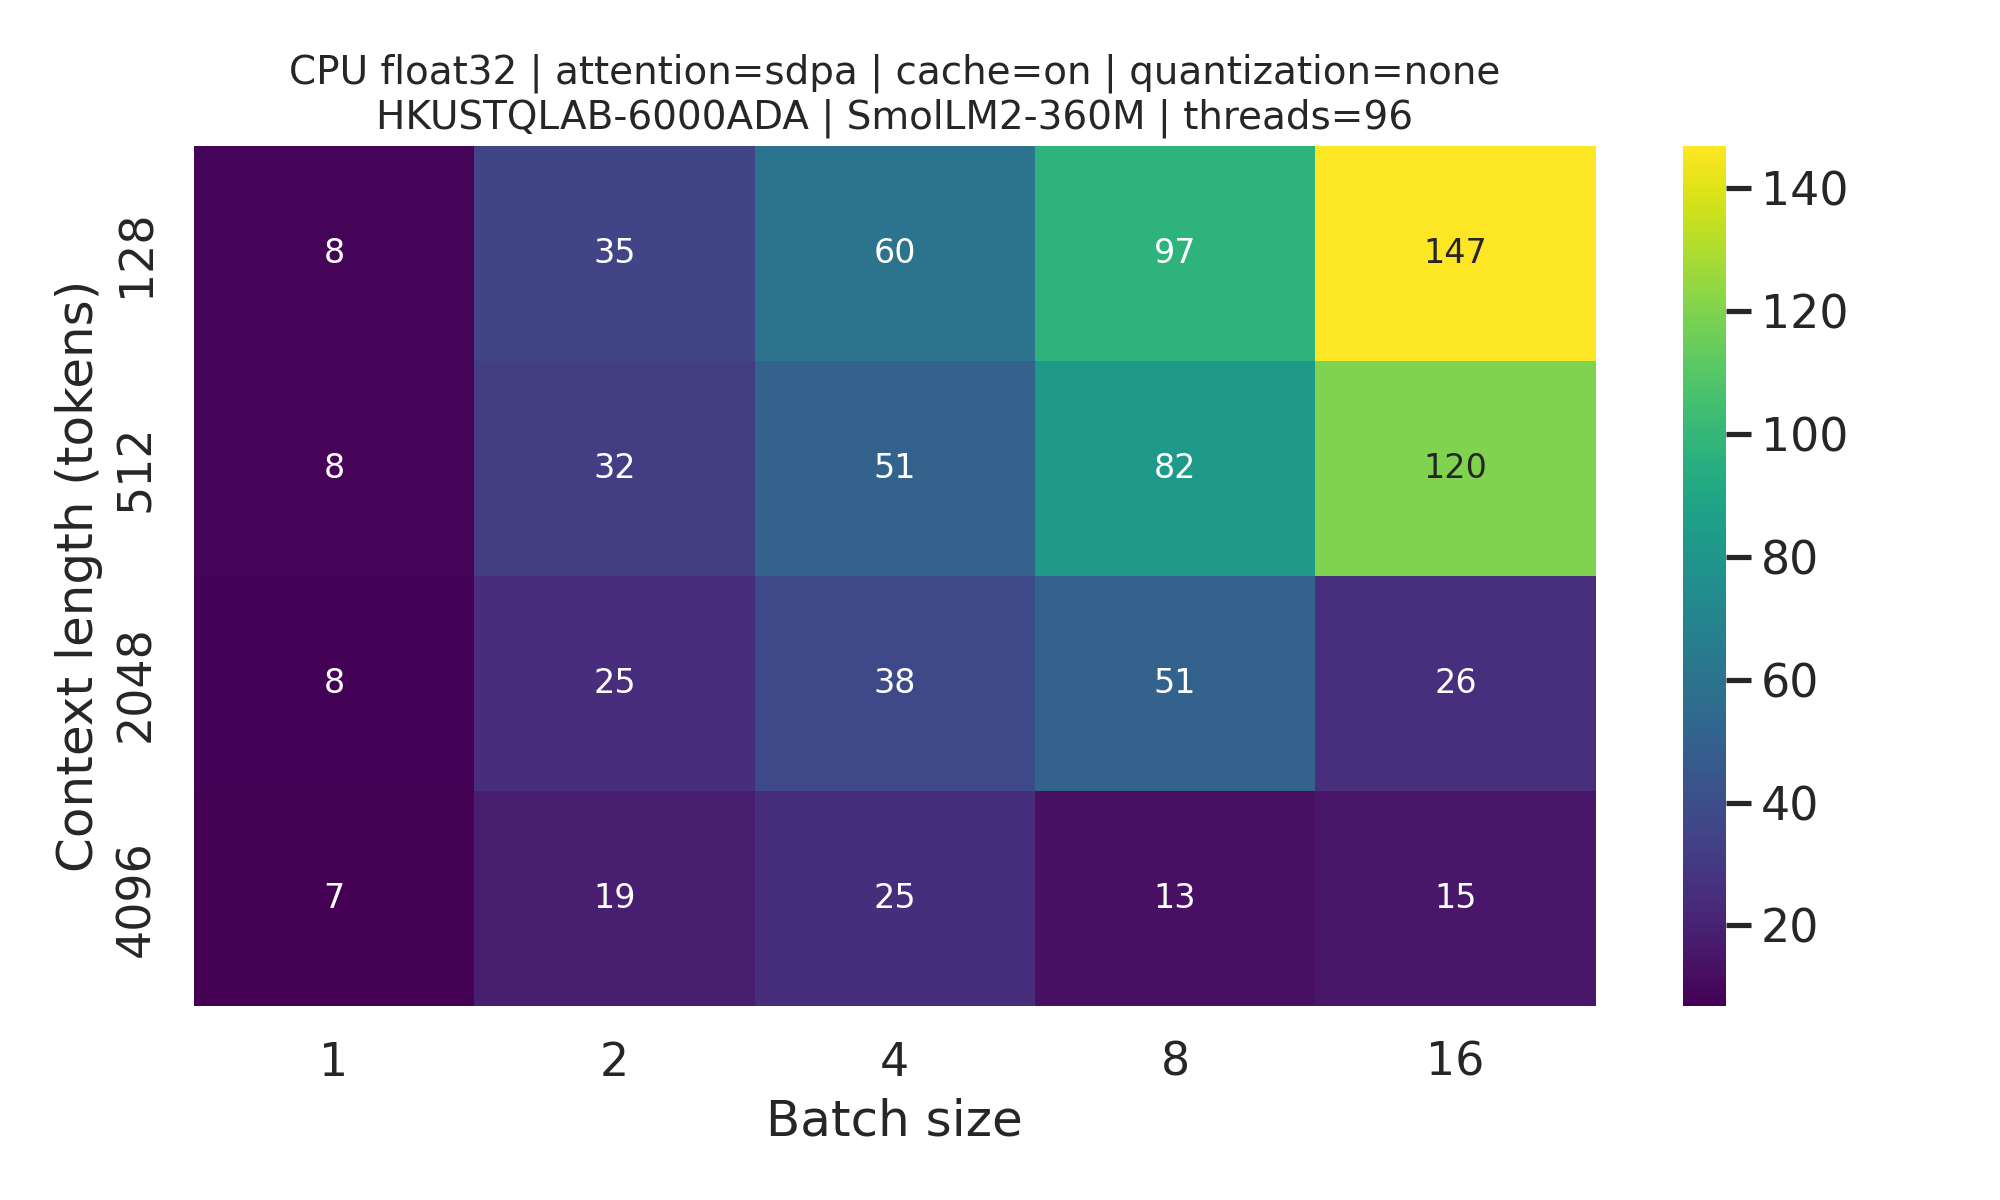
\includegraphics[width=\linewidth]{tps_heatmap_HKUSTQLAB-6000ADA_cpu_float32_sdpa_cache-on_none_SmolLM2-360M.png}\\[-1mm]
    \footnotesize (a) CPU FP32, batches 1--16
  \end{minipage}\hfill
  \begin{minipage}[t]{0.49\textwidth}
    \centering
    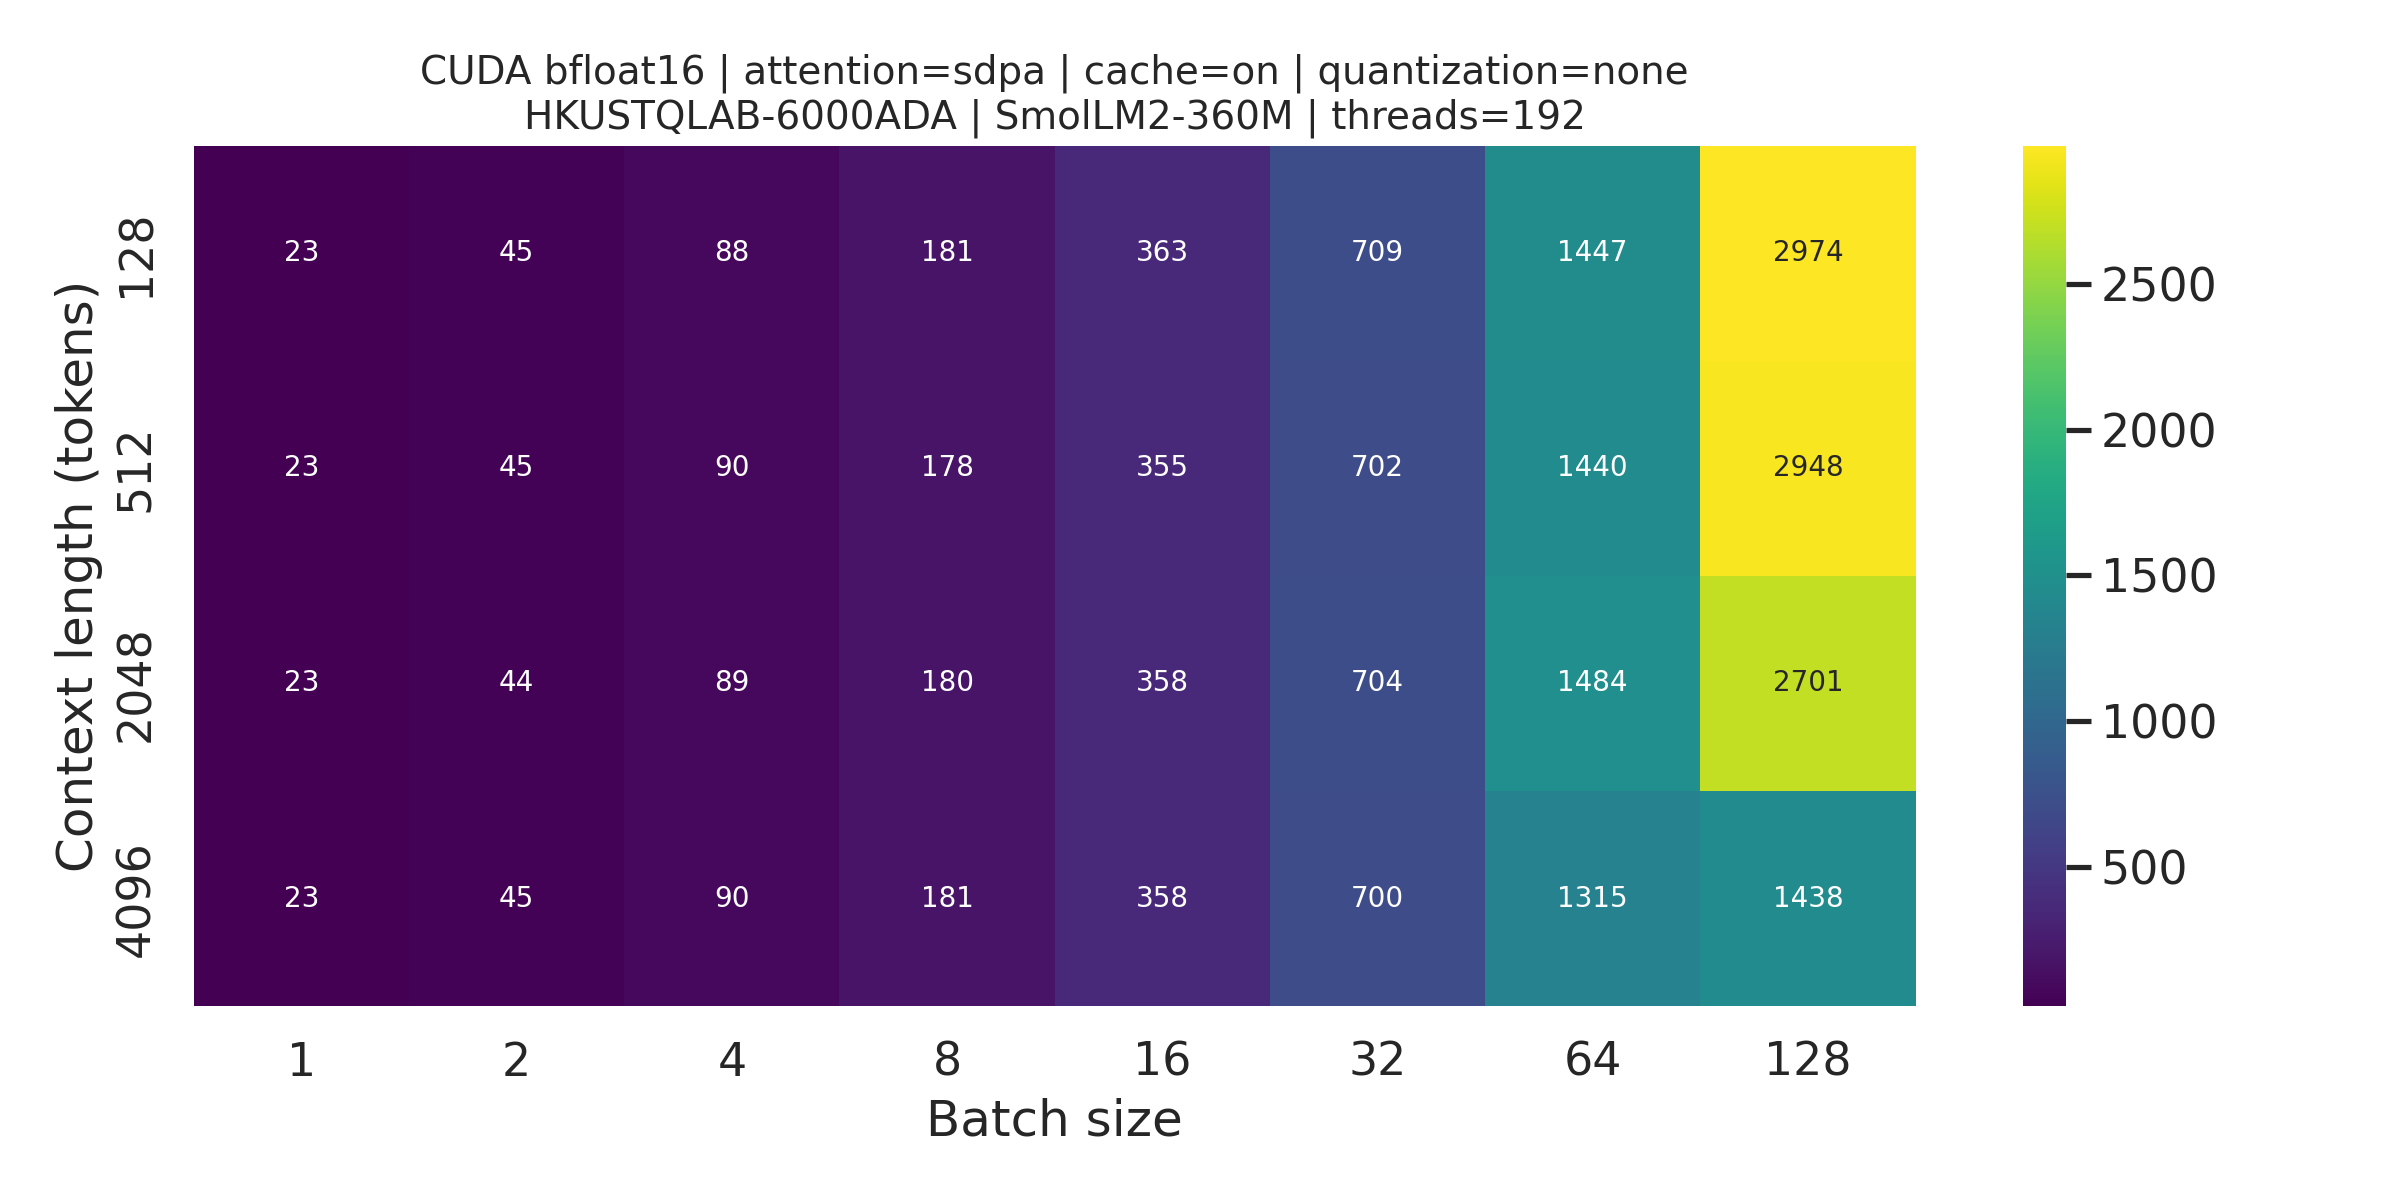
\includegraphics[width=\linewidth]{tps_heatmap_HKUSTQLAB-6000ADA_cuda_bfloat16_sdpa_cache-on_none_SmolLM2-360M.png}\\[-1mm]
    \footnotesize (b) RTX 6000 Ada BF16, batches 1--128
  \end{minipage}
  \caption{Corrected median decode-throughput surfaces. Long context moves
  the CPU knee to smaller batches, whereas the GPU continues to gain
  throughput until the edge of most tested grids.}
  \label{fig:baseline}
\end{figure*}

\subsection{Attention and Cache Crossovers}

Table~\ref{tab:interventions} summarizes the intervention effects. On CPU,
eager/SDPA median TTFT grows from 1.00$\times$ at 128/1 to 6.23$\times$ at
4096/4; TPOT grows from 1.11$\times$ to 4.09$\times$. On GPU, the TTFT ratio
grows from 1.40$\times$ to 9.34$\times$, while TPOT stays near a
1.30$\times$ eager penalty. The increasing long-context advantage and the
observed fused kernel support an operator-level explanation rather than a
label-only comparison.

Caching shows a workload-dependent crossover. On CPU, cache-off median TPOT
is 1.85--17.62$\times$ cache-on at five repeated points. The single 2048/8
boundary reaches 88.99$\times$ and takes 891.7~s; it is reported as a
boundary, not a percentile. On GPU, cache-off is 1--5\% faster at five
smaller loads, then becomes 4.22$\times$ slower at 2048/8. For this 360M
model, cache bookkeeping can exceed recomputation before the
sequence--batch product becomes sufficiently large. Production systems
therefore need explicit KV-memory management~\cite{pagedattention}, although
our synchronous harness does not implement PagedAttention or request
scheduling.

\begin{table}[t]
\caption{Normalized Intervention Effects}
\label{tab:interventions}
\centering
\small
\setlength{\tabcolsep}{3.5pt}
\begin{tabularx}{\columnwidth}{@{}lYY@{}}
\toprule
\textbf{Study} & \textbf{Measured effect} & \textbf{Interpretation} \\
\midrule
SDPA &
4096/4 TTFT: 6.23$\times$ CPU, 9.34$\times$ GPU &
Clear long-context win; fused CUDA path verified. \\
KV cache &
GPU off/on TPOT: 0.95--0.99$\times$ at small loads; 4.22$\times$ at 2048/8 &
Bookkeeping versus recomputation. \\
CPU W8A8 &
TPS 1.27--2.49$\times$; RSS 1.12--1.66$\times$ &
Speed improvement, not resident-memory reduction. \\
\bottomrule
\end{tabularx}
\end{table}

\subsection{Quantization, Memory, and Quality}

CPU W8A8 increases median TPS by 1.27--2.49$\times$ across four points, but
peak RSS is 1.12--1.66$\times$ the native path. The tested eager dynamic
quantization path is therefore a speed optimization, not a resident-memory
optimization. The quality cost is substantial: WikiText-2 perplexity rises
from 11.27 to 44.16, while full ARC-Easy accuracy falls from 56.44\% to
42.21\% (normalized: 49.12\% to 38.97\%). Native HellaSwag accuracy is
42.83\%, or 56.88\% with standard length normalization, over 10,042 examples
(approximately 0.49 percentage-point standard error).

The GPU TorchAO path is retained as a negative diagnostic. Profiling confirms
225 \texttt{aten::\_int\_mm} calls and 224 Ampere INT8 GEMMs, but also 9,025
device-to-host scalar transfers during one 128/1 prefill. Throughput is only
about 0.21 TPS, so we make no full-grid GPU W8A8 speed claim. Functional INT8
execution is not sufficient evidence of an efficient end-to-end serving
path.

\begin{table}[t]
\caption{CPU W8A8 Quality}
\label{tab:quality}
\centering
\small
\begin{tabular}{@{}lrrr@{}}
\toprule
\textbf{Metric} & \textbf{Native} & \textbf{W8A8} & \textbf{Change} \\
\midrule
WikiText-2 PPL & 11.27 & 44.16 & +32.89 \\
ARC-Easy acc. & 56.44\% & 42.21\% & -14.23 pp \\
ARC-Easy acc.\_norm & 49.12\% & 38.97\% & -10.14 pp \\
\bottomrule
\end{tabular}
\end{table}

\subsection{Synthesis and Limitations}

The resulting selection map is workload-shaped. Short, small GPU loads are
overhead-sensitive and may not benefit from cache state. Larger batches
increase utilization until context-driven latency and activation/KV memory
tighten the frontier. Long-context prefill strongly favors SDPA. Long,
batched decode favors caching. CPU W8A8 is attractive only when its speedup
justifies higher RSS and the measured quality loss is acceptable, or when a
better calibration and quantization recipe restores accuracy.

These are synchronous, model-only measurements. They exclude tokenization,
networking, continuous batching, admission control, request queues, prefix
sharing, and multi-tenant effects. The study uses one small model, one CPU
platform, one GPU model, and one main framework. Future work should repeat
the region map with a production scheduler, larger models, static or compiled
cache paths, and alternative quantization recipes.

\newpage
\section{Contribution Statement}

Hanxiao led the benchmark framework, reproducibility controls, CPU
experiments, and data correction and validation. Haiyang Peng led GPU
execution, operator/cache/quantization studies, and quality evaluation. Both
authors jointly designed the experiment, interpreted results, reviewed
artifacts, and prepared the report and presentation.

\section{AI-Use Acknowledgment}

OpenAI Codex was used for repository planning, implementation and debugging
assistance, consistency audits, and drafting and editing the presentation and
report. The authors executed the experiments, reviewed generated changes,
verified raw and processed results against manifests and profiler evidence,
reran tests, and remain responsible for all claims. AI-generated text or code
was not treated as experimental evidence.

\bibliographystyle{IEEEtran}
\bibliography{references}

\end{document}
